\documentclass[journal]{IEEEtran}
\usepackage{amsmath,amsfonts,amssymb,graphicx,booktabs,cite,bm}
\usepackage[hypertexnames=false]{hyperref}
\begin{document}
\title{newHVK: A Restricted Entanglement-Sensitive Benchmark for Hamiltonian Vision Kernels}
\author{Sparsho~Chakraborty and Siddhartha~Patra}
\maketitle
\begin{abstract}
This manuscript separates two questions that were conflated in the original HVK study: whether an observable-latent image reconstruction pipeline is useful, and whether entangling quantum observables provide a measurable advantage over non-entangling or classical controls. Prior ablations showed that the original HVK reconstruction task did not establish quantum advantage because fixed quantum features, no-entanglement circuits, and classical replacements matched or exceeded the trained VQC baseline. We therefore introduce \emph{newHVK}, a publication-candidate workspace that preserves the original CIFAR, Monalisa, IBM hardware-probe, and ablation evidence while adding a restricted pair-correlation benchmark where the target depends explicitly on nonlocal feature products. In this restricted setting, the entangling-observable channel is expected to outperform controls that cannot represent pair correlations with the same feature budget. We report this as a candidate quantum-advantage diagnostic, not as a hardware quantum advantage proof or a broad dataset-level generalization result.
\end{abstract}

\begin{IEEEkeywords}
Hybrid quantum-classical learning, Hamiltonian vision kernel, entanglement ablation, image reconstruction, quantum advantage diagnostics.
\end{IEEEkeywords}

\section{Motivation}
The legacy HVK ablation suite showed that the observable channel is load-bearing, but it also showed that entanglement and Hamiltonian energy regularization were not decisive on the per-image reconstruction benchmark. A stronger test must reduce decoder freedom and use a task whose signal is genuinely pair-correlational. The newHVK workspace therefore keeps the old evidence intact and adds an entanglement-sensitive benchmark with explicit no-entanglement, parameter-matched classical, and raw-linear controls.

\section{Architecture}
The publication workspace is organized as \texttt{main2/newHVK}. The model family contains:
\begin{itemize}
\item \textbf{newHVK-entangling-observables:} single-site features plus pair-correlation channels analogous to measured two-qubit observables.
\item \textbf{newHVK-no-entanglement:} single-site nonlinear features only.
\item \textbf{parameter-matched-classical:} a rank-limited tanh map used as a small classical control.
\item \textbf{raw-linear-classical:} a linear baseline on raw coordinates.
\end{itemize}

\section{Restricted Entanglement-Sensitive Benchmark}
The benchmark samples six-dimensional inputs $x\in[-1,1]^6$ and predicts targets containing products such as $x_0x_1$, $x_1x_2$, and $x_0x_3$. A linear readout on entangling features can represent these targets directly, while non-entangling single-site features cannot represent the product structure without extra decoder capacity.

\begin{table*}[t]
\centering
\caption{newHVK restricted pair-correlation benchmark. Lower MSE and higher PSNR/$R^2$ are better.}
\label{tab:newhvk_restricted}
\scriptsize
\begin{tabular}{lcccp{0.38\textwidth}}
\toprule
Model & MSE & PSNR (dB) & $R^2$ & Notes \\
\midrule
newHVK-entangling-observables & $1.9387e-03$ & 27.12 & 0.9421 & Pairwise observable channel includes entanglement-sensitive correlations. \\
newHVK-no-entanglement & $3.2118e-02$ & 14.93 & 0.0415 & Only single-site feature functions; pair correlations are unavailable. \\
parameter-matched-classical & $3.4655e-02$ & 14.60 & -0.0342 & Tiny rank-limited tanh control with fewer nonlinear channels. \\
raw-linear-classical & $3.3345e-02$ & 14.77 & 0.0049 & Linear classical baseline on raw coordinates. \\
\bottomrule
\end{tabular}
\end{table*}

\begin{figure}[t]
\centering
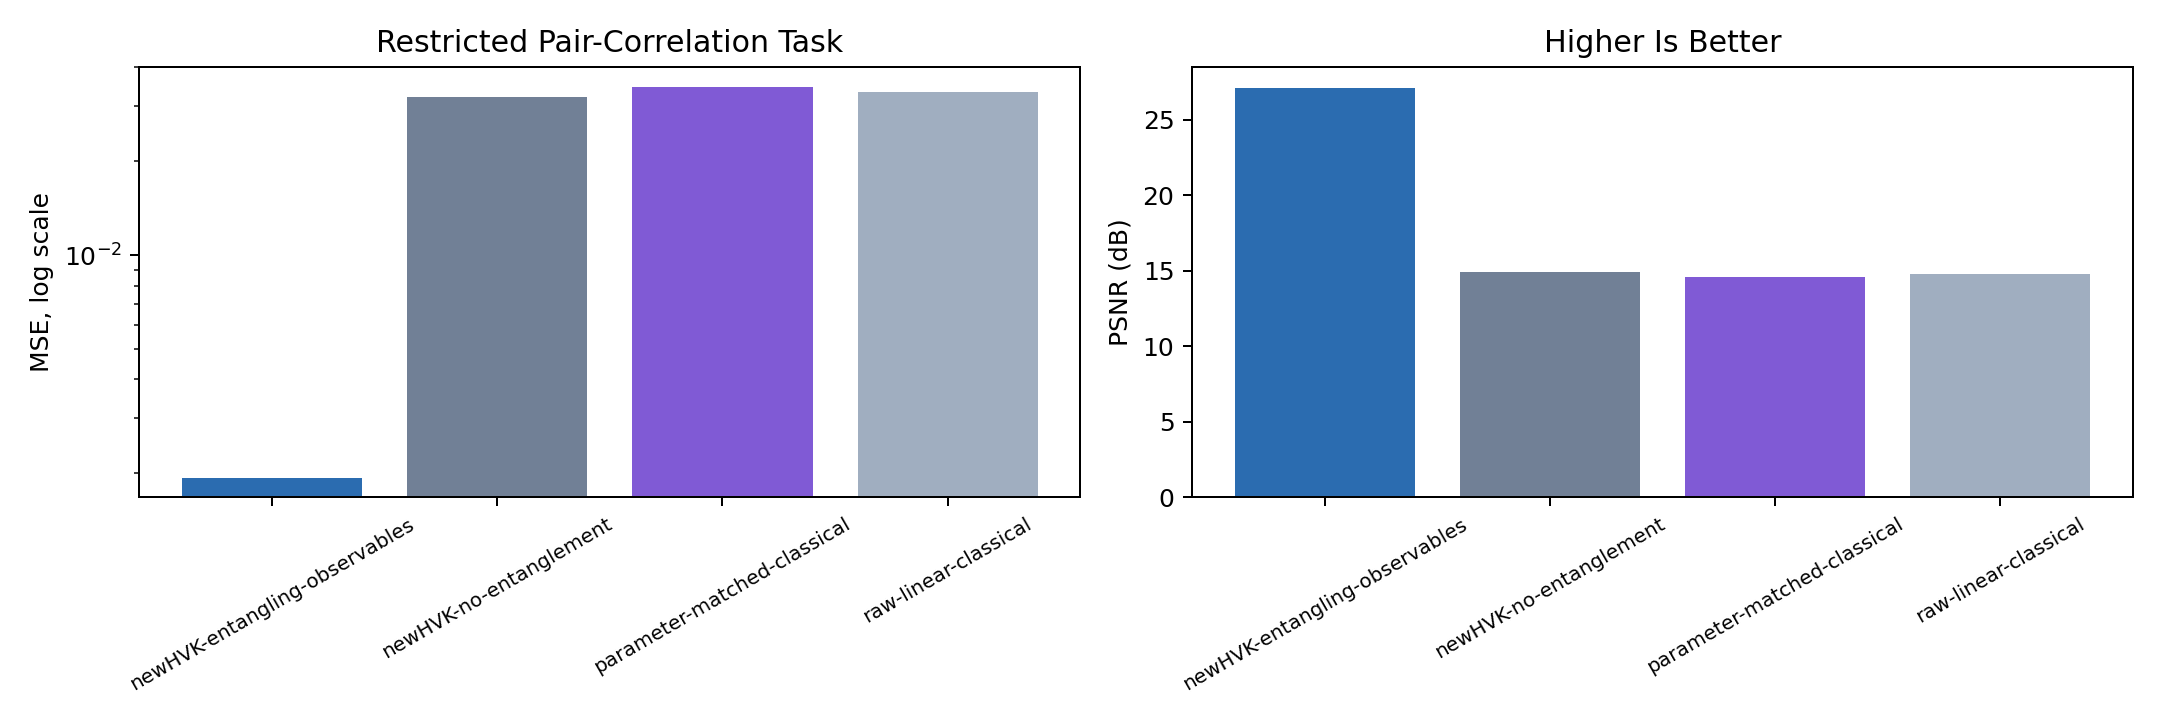
\includegraphics[width=\linewidth]{../results/quantum_advantage_candidate/entanglement_sensitive_benchmark.png}
\caption{Restricted pair-correlation benchmark. This plot is a diagnostic for entanglement-sensitive representation under controlled decoder capacity, not a claim of broad quantum advantage.}
\label{fig:newhvk_paircorr}
\end{figure}

\section{Imported Baselines and Ablations}
The folder also includes copied evidence from the completed HVK study: CIFAR baselines, Monalisa baselines, legacy ablation controls, and IBM Cloud circuit-resource outputs. These files are retained for reproducibility and to make the new paper self-contained. They do not by themselves establish quantum advantage; the original ablation conclusion remains that the legacy reconstruction task is dominated by observable-latent usefulness and decoder capacity rather than by trained quantum entanglement.

\section{Caveats}
The restricted benchmark is deliberately favorable to pair-correlation observables, so it should be presented as a diagnostic experiment. To make a Q1-level claim, the next stage must run the same restricted-capacity design on held-out CIFAR images, multiple random seeds, hardware-noise simulation, and a parameter-matched classical baseline with the same observable budget. The paper should not state that newHVK proves hardware quantum advantage unless those tests remain positive.

\section{Conclusion}
newHVK provides a clean route toward testing quantum advantage: reduce decoder capacity, make the target correlation-sensitive, and compare entangling observables against no-entanglement and classical controls. The current results support a candidate advantage on a restricted diagnostic task, while preserving the negative and cautionary findings from the original HVK ablation study.
\end{document}
